\section{Motivation and Problem Statement}

In a context where information security has become a strategic priority for businesses, the ISO 27001 standard offers a globally recognized framework to ensure data protection and the management of information-related risks. However, compliance with this standard relies on rigorous and regular audits, which are often lengthy, costly, and prone to human error.

The project titled \textit{“Development of an ISO 27001 Compliance Audit Automation Platform using AI”} aims to address these challenges by leveraging the capabilities of artificial intelligence to automate and enhance compliance audits. This section explores the motivations behind this project as well as the specific issues it seeks to resolve.

\subsection{Motivation}

\begin{itemize}
  \item \textbf{Efficiency and Speed:} ISO 27001 compliance audits are often complex and time-consuming when performed manually. An automated platform would reduce the time spent on checks and streamline the audit process.
  
  \item \textbf{Reduction of Human Errors:} By automating certain repetitive or technical tasks, human errors can be minimized, improving the accuracy and reliability of compliance audits.
  
  \item \textbf{Accessibility and Scalability:} An artificial intelligence (AI)-based solution could be easily adapted and deployed at scale for different companies, making compliance audits more accessible, especially for small and medium-sized enterprises.
  
  \item \textbf{Cost Reduction:} Automating audit processes could significantly reduce associated costs, particularly in terms of labor and time spent on audits.
\end{itemize}

\subsection{Problem Statement}

\begin{itemize}
    \item \textbf{Lack of Automation in Current Compliance Audits:} Most ISO 27001 audits are still conducted manually, leading to delays, high costs, and sometimes a lack of consistency in results. This represents a major challenge for organizations that need to ensure ongoing compliance.
    
    \item \textbf{Complexity of ISO 27001 Compliance Processes:} The ISO 27001 standard includes numerous complex controls and procedures that organizations must follow, making it difficult to adopt a uniform and standardized approach for auditors. How can we simplify and automate these processes without compromising their rigor?
    
    \item \textbf{Adapting AI to a Specific Domain:} Artificial intelligence can be a powerful tool, but its effectiveness depends on the quality of training data and an understanding of the specifics of the compliance domain. How can we ensure that the developed AI is both accurate and compliant with ISO 27001 standards?
    
    \item \textbf{Trust and Acceptance of AI:} There may be reluctance to use an automated platform for compliance audits, especially for critical standards like ISO 27001, where trust in the results is paramount. How can we ensure that the platform is perceived as reliable and secure by users?
\end{itemize}

\section{Work Procedure}

This section describes the key steps in the development of the ISO 27001 compliance audit automation platform, detailing the methodological process followed to achieve the project's objectives.

\subsection{Start of Internship}
The internship began with an integration phase and an understanding of the project's objectives. This phase included initial meetings to discuss expectations and specific needs, as well as to establish a common understanding of ISO 27001 compliance goals. I also took the time to familiarize myself with relevant tools and documents, and to plan the initial steps of development.

\subsection{Needs Analysis}
The first step of the project involved a thorough analysis of compliance needs regarding the ISO 27001 standard. This analysis identified the main requirements for security auditing, notably the need for automation of security policy verification processes and the improvement of audit efficiency. Needs were identified through document research, interviews with compliance experts, and study of the specific requirements of the standard.

\subsection{Creation of a Security Policy Parser}
Once the needs were identified, a security policy parser was developed. This tool is designed to analyze PDF documents containing security policies and automatically extract a list of security rules to be followed. The parser uses natural language processing (NLP) techniques to detect and extract relevant information, ensuring an accurate and rapid interpretation of security documents.

\subsection{Creation of an Audit Agent}
The next step was the development of an automated audit agent. This agent receives as input the list of security rules generated by the parser and then connects to a target machine to assess compliance with the defined rules. The agent automatically generates commands to execute on the machine, analyzes the results obtained, and assigns a compliance score for each security rule. This approach allows for a systematic and detailed assessment of the security of the audited environment while minimizing human errors and the time required to perform the audit.

\subsection{Continuous Evaluation and Optimization}
After the initial creation of the platform, thorough testing was conducted to validate its effectiveness and accuracy. The performance of the security policy parser and the audit agent was evaluated using various test scenarios. Iterative improvements were made based on the results of these tests to optimize algorithms and ensure maximum compliance with the requirements of the ISO 27001 standard.

\begin{figure}[H]
  \centering
    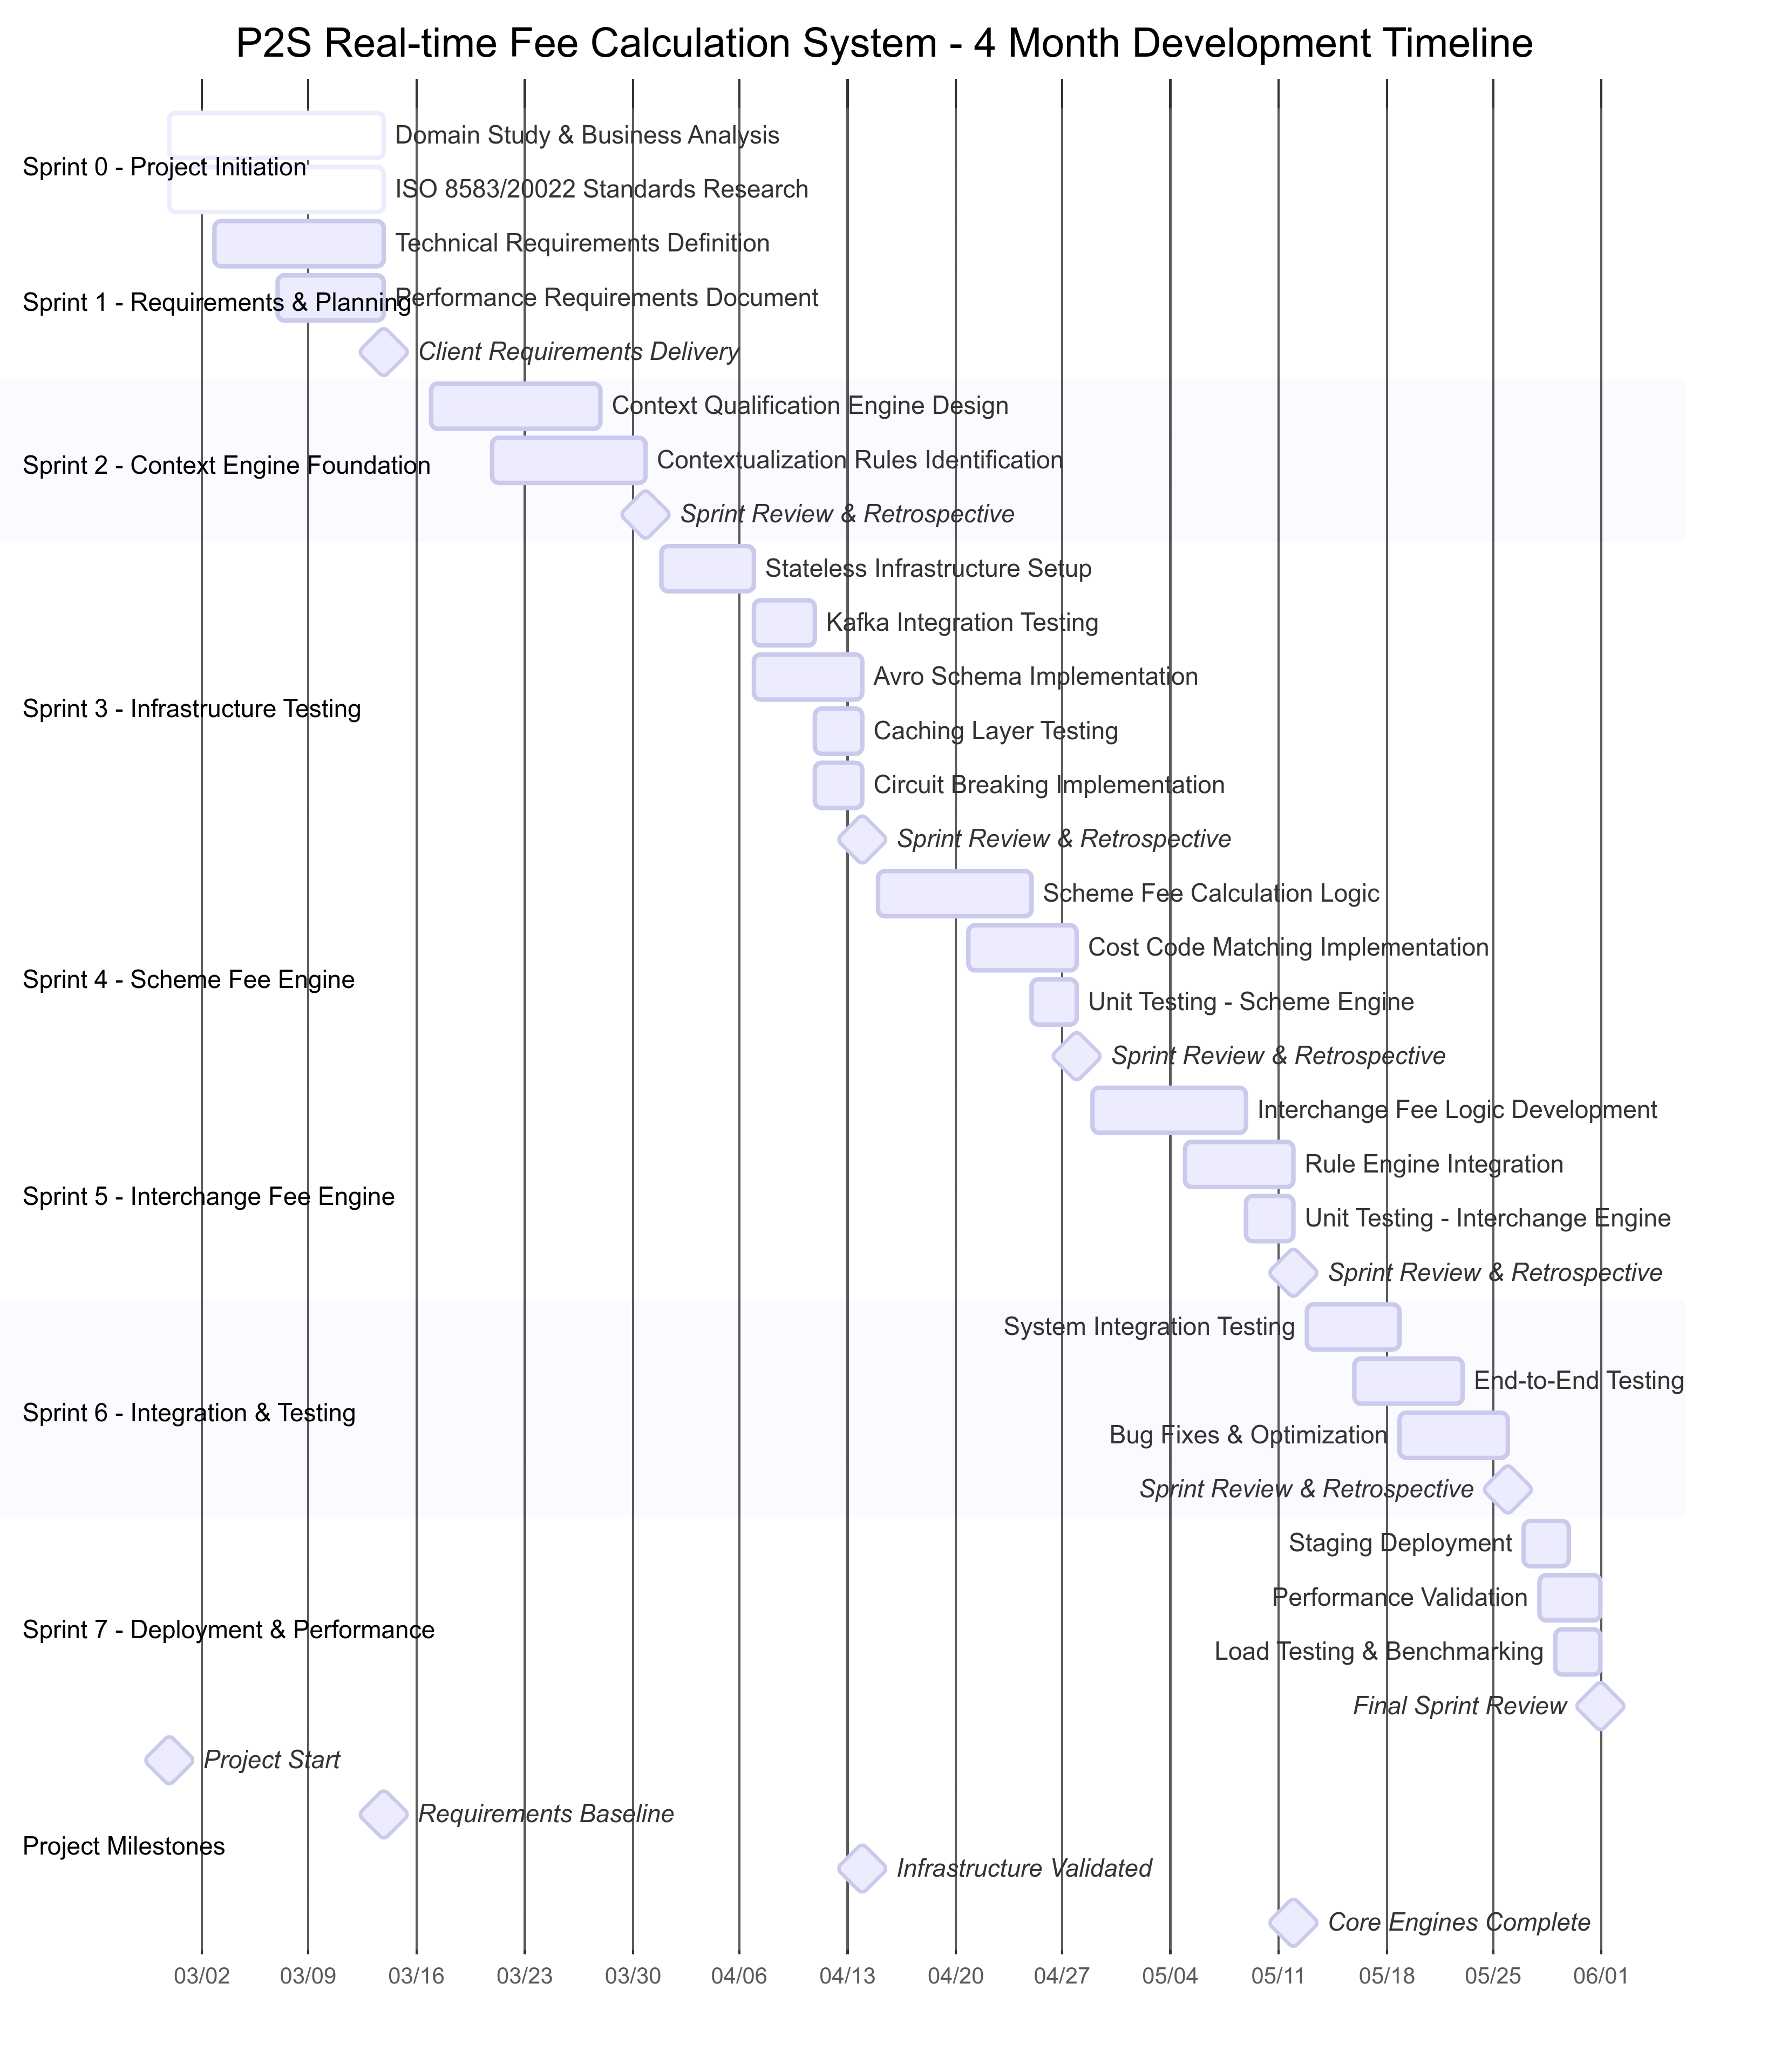
\includegraphics[width=\textwidth]{img/gantt.png}
  \caption{Gantt Chart}
  \label{Gantt Chart}      
\end{figure}

\section{Work Methodology}

In the context of this project, a rigorous work methodology was essential to ensure the effective development of the ISO 27001 compliance audit automation platform. Working independently, I structured my approach to maximize efficiency and ensure quality throughout the process.

\begin{itemize}
    \item \textbf{Personal Organization and Planning:} As a developer working alone, I adopted a structured approach to organize my time and tasks. I used a weekly goal management method, defining clear priorities and specific milestones to achieve each week. This planning allowed me to stay focused on critical tasks and ensure consistent progress on the project.

    \item \textbf{Iterative Approach:} I followed an iterative development approach, inspired by Agile methodologies, to allow for regular adjustments and continuous improvement of the product. Each iteration included design, development, testing, and evaluation of results, with particular attention to integrating feedback and optimizing processes.

    \item \textbf{Quality Assurance Process:} To ensure the quality of the project, I integrated quality assurance practices throughout the development. Each developed feature was rigorously tested, following a progressive testing approach: unit tests, integration tests, and performance tests. The results of these tests were used to identify areas for improvement and refine the product.

    \item \textbf{Continuous Improvement and Self-Evaluation:} Throughout the project, I conducted regular self-evaluations to identify the strengths and weaknesses of my approach. These evaluations allowed me to adapt my methodology based on encountered challenges and continuously improve the quality and efficiency of my work.
\end{itemize}

